\section{Introduction}
\label{sec:introduction}

In this laboratory, we analysed in a theoretical approach as well as using software simulation, a Pass-band Filter using an Operational Amplifier (OPAMP).
It was composed of three different stages: a High Pass Stage (with the objective of, as it name expresses, passing signals with high frequencies and cutting the ones with low frequencies, as we'll discuss in greater detail), an Amplification Stage (whose objective is, using the OPAMP, to amplify the signal) and, finally, a Low Pass Stage (that given the amplified signal from the previous stages, allows the low frequencies to pass and cuts off the high ones). In this report, a software simulation and theoretical analysis will be stacked up against each other. This assignment allowed us to deal with important concepts such as the \textbf{OPAMPs} - its input and output impedances, as well as gain and operation. In Figure \ref{fig:circuitol5} the stated circuit is presented. 

Also, regarding the OPAMP it is important to notice that the model $\mu$A741 from Texas Instruments was the chosen one. 

After the theoretical analysis, the circuit is analysed by computational simulation tools, via \textit{Ngspice}, and the results are compared to the theoretical results obtained, in Section \ref{sec:analysis}. The conclusions of this study are outlined in Section \ref{sec:conclusion}.

\begin{figure}[h] \centering
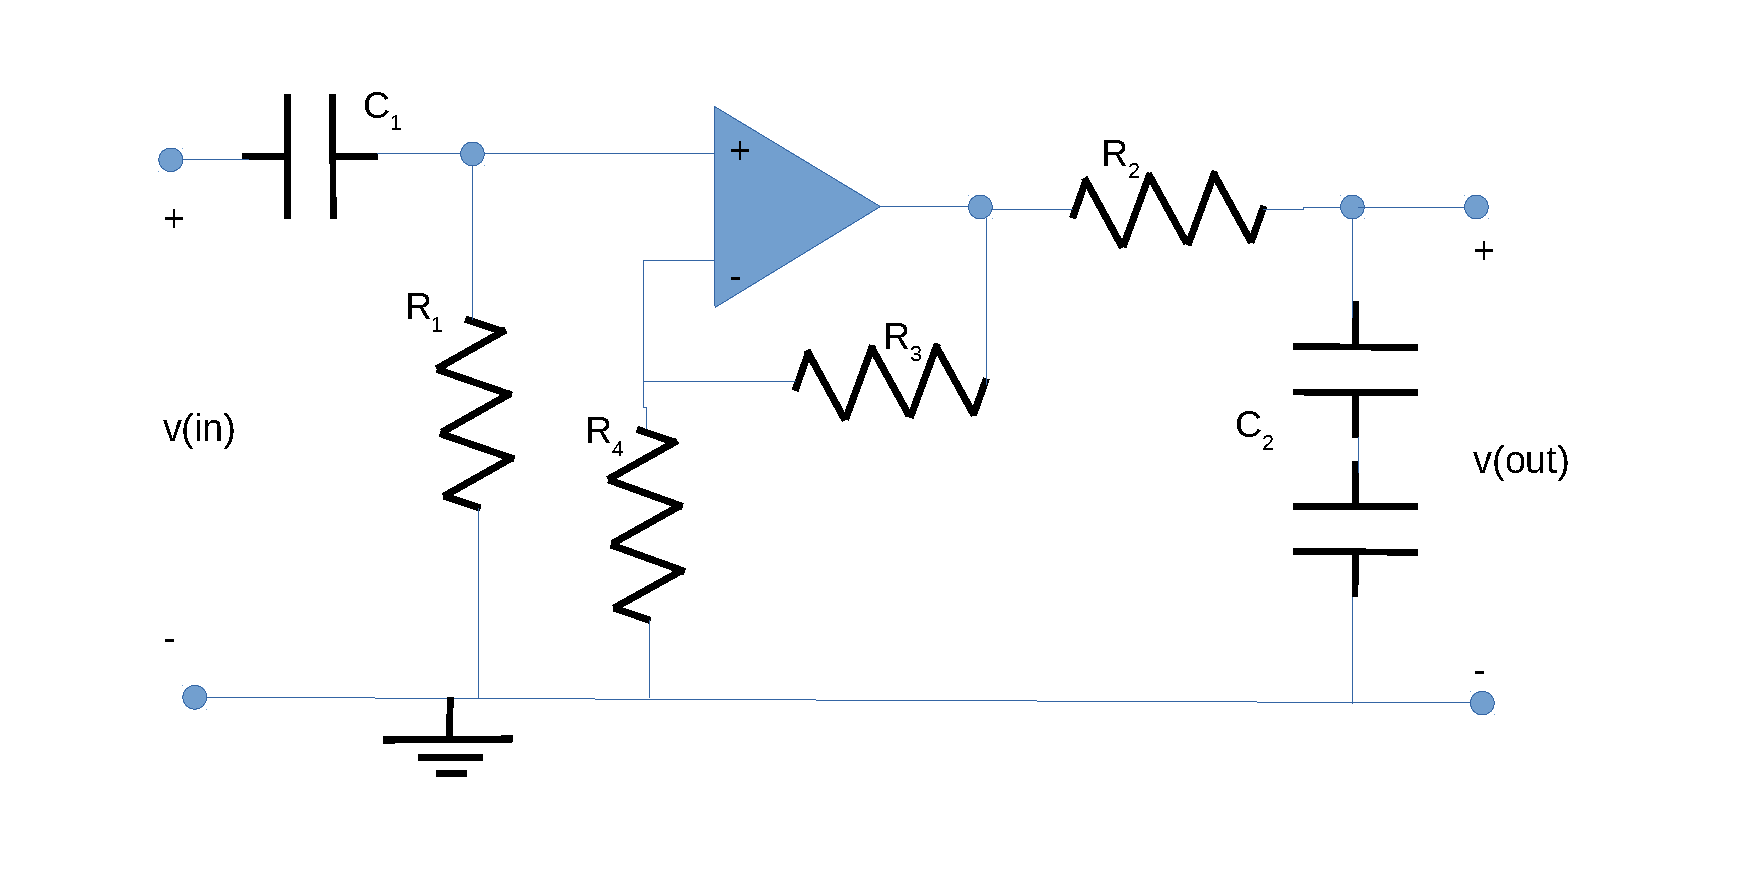
\includegraphics[width=1\linewidth]{circuitl5_old.pdf}
\caption{Active Passband Filter}
\label{fig:circuitol5}
\end{figure}

\clearpage
